% template: apssamp.tex


\documentclass[
    floatfix,  % fix: "LaTeX: A float is stuck (cannot be placed); try class option [floatfix]."
    reprint,
    amsmath,
    amssymb,
    aps,
    %superscriptaddress,
    %groupedaddress,
    %unsortedaddress,
    %runinaddress,
    %frontmatterverbose,
    %preprint,
    %preprintnumbers,
    %nofootinbib,
    %nobibnotes,
    %bibnotes,
    %pra,
    %prb,
    %rmp,
    %prstab,
    %prstper,
]{revtex4-2}


% \usepackage{gensymb}
\usepackage{graphicx}% Include figure files
\usepackage{dcolumn}% Align table columns on decimal point
\usepackage{bm}% bold math
%\usepackage{hyperref}% add hypertext capabilities
% \usepackage[mathlines]{lineno}% Enable numbering of text and display math
%\linenumbers\relax % Commence numbering lines

%\usepackage[showframe,%Uncomment any one of the following lines to test
%%scale=0.7, marginratio={1:1, 2:3}, ignoreall,% default settings
%%text={7in,10in},centering,
%%margin=1.5in,
%%total={6.5in,8.75in}, top=1.2in, left=0.9in, includefoot,
%%height=10in,a5paper,hmargin={3cm,0.8in},
%]{geometry}



%%% USER ADDED PACKAGES

% user added packages
\usepackage{xfrac}
\usepackage{mathtools}
\usepackage{subcaption}
\usepackage{siunitx}
\usepackage[LGR,T1]{fontenc}
\usepackage{textcomp}  % for \texteuro, \textperthousand, etc.
\usepackage{lmodern}
\usepackage{amsmath}
\usepackage{booktabs}    % nicer rules
\usepackage{multirow}    % for multirow cells

\DeclarePairedDelimiter\bra{\langle}{\rvert}
\DeclarePairedDelimiter\ket{\lvert}{\rangle}
\DeclarePairedDelimiterX\braket[2]{\langle}{\rangle}{#1\,\delimsize\vert\,\mathopen{}#2}
\DeclareMathAlphabet{\mathgtt}{LGR}{cmtt}{m}{n}
%%% COMMANDS


\newcommand{\half}{$\sfrac{1}{2}$ }
\newcommand{\pauliz}{
    \begin{pmatrix}
        1 & 0 \\
        0 & -1
\end{pmatrix}}
\newcommand{\halfpi}{\frac{\pi}{2}}
\newcommand{\taucode}{\mathgtt{t}}






















% ---------------------------------------------------------------------------- %
%                                    HEADER                                    %
% ---------------------------------------------------------------------------- %

\begin{document}

\preprint{APS/123-QED}

\title{Nuclear Magnetic Resonance -- An Overview}

\author{Ali Ahmed}
\author{Zain Kamal}
\author{Neil Mandar}

\affiliation{
    Department of Physics \& Astronomy, Rutgers University
}

\date{\today}

\begin{abstract}
    This report summarizes our investigation of pulsed nuclear magnetic resonance (NMR) using the TeachSpin spectrometer. Building on the principles of Larmor precession and the quantum-mechanical behavior of spin-$\half$ nuclei, we examined the response of magnetic moments when subjected to time-dependent radio frequency (RF) pulses. We began with a theoretical framework covering key concepts such as the net magnetization arising from the Boltzmann population difference and the associated longitudinal ($T_1$) and transverse ($T_2$) relaxation processes. In our experiments, specially-tuned $\halfpi$ and $\pi$ pulses were applied to tip and invert the magnetization, thereby generating free induction decay (FID) signals and spin echoes. A simulation model incorporating the exponential decay of echo amplitudes provided a basis for comparing the expected with the observed signal features. Data analysis of envelope decay yielded $T_1$ and $T_2$ times for mineral oil, water, and glycerol. Our study demonstrates the successful application of pulsed NMR techniques in measuring relaxation times, validating both the theoretical description and the simulation model.
\end{abstract}

\maketitle

%\tableofcontents




% ---------------------------------------------------------------------------- %
%                                     INTRO                                    %
% ---------------------------------------------------------------------------- %

\section{\label{sec:intro}Introduction and Theoretical Description}

The study of nuclear magnetic resonance (NMR) utilizes weak magnetic fields to affect the nuclei of atoms in a strong magnetic field. Under certain conditions, atoms will exhibit ``resonance,'' causing the observation of a transient magnetic field as nuclei relax back to their equillibrium state.








% ---------------------------------------------------------------------------- %

\subsection{\label{subsec:larmor} Larmor Precession}

We will start with the phenomena of Larmor precession, occuring when atoms are placed in a strong magnetic field.
Larmor precession most readily occurs when the nucleus has a net magnetic moment i.e. there is an odd number of nucleons (protons and neutrons), producing a spin $\half$ system (e.g. $^1H$, $^{13}C$, $^{19}F$, etc.). In this case, the magnetic dipole moment $\mu$ of the nucleus is described as

\begin{equation}
    \vec{\mu} = \gamma \vec{S}
\end{equation}

where $\vec{S}$ denotes the spin vector and $\gamma$ is a constant known as the gyromagnetic ratio (which differs depending on the type of nucleus). Under a magnetic field, the energy of this system reads

\begin{equation}
    E = -\vec{\mu} \cdot \vec{B_0}
\end{equation}

where we denote $B_0$ the external magnetic field. This yields the Hamiltonian

\begin{equation}\label{eqn:base-hamiltonian}
    H = -\gamma \vec{B_0} \cdot S
\end{equation}

where $S$ is the Pauli spin operator $S = (\sigma_x, \sigma_y, \sigma_z)$. Let us orient our magnetic field against the z-axis, such that

\begin{equation}
    \vec{B_0} = B_0 \hat{z}
\end{equation}

and the Hamiltonian now reads

\begin{equation}\label{eqn:hamiltonian}
    H = -\frac{\hbar}{2} \gamma B_0  \pauliz
\end{equation}

The Hamiltonian has eigenstates

\begin{equation}
    \ket{\pm} : E_\pm = \mp \frac{\hbar}{2} \gamma B_0
\end{equation}

These eigenstates correspond to nuclei aligned either parallel or antiparallel to the magnetic field $B_0$. We will use these vectors $\ket{\pm}$ as our basis. We can evolve these stationary states with the time-dependent Schr\"odinger equation and then calculate the expectation of each of our Pauli matrices to obtain

\begin{align*}
    \langle S_x \rangle &= \frac{\hbar}{2} \sin(\theta)\cos(\gamma B_0 t)\\
    \langle S_y \rangle &= \frac{\hbar}{2} \sin(\theta)\sin(\gamma B_0 t)\\
    \langle S_z \rangle &= \frac{\hbar}{2} \cos(\theta)
\end{align*}

These equations are the classical precession equations; our spin vector will precess about the magnetic field at a constant frequency
\begin{equation}
    \omega_0 = \gamma B_0
\end{equation}

This frequency is known as the \textbf{Larmor frequency}, and $\theta$ indicates the angle between $\vec{\mu}$ and $\vec{B_0}$. \cite{griffiths}

\begin{figure}[htbp]
    \centering
    {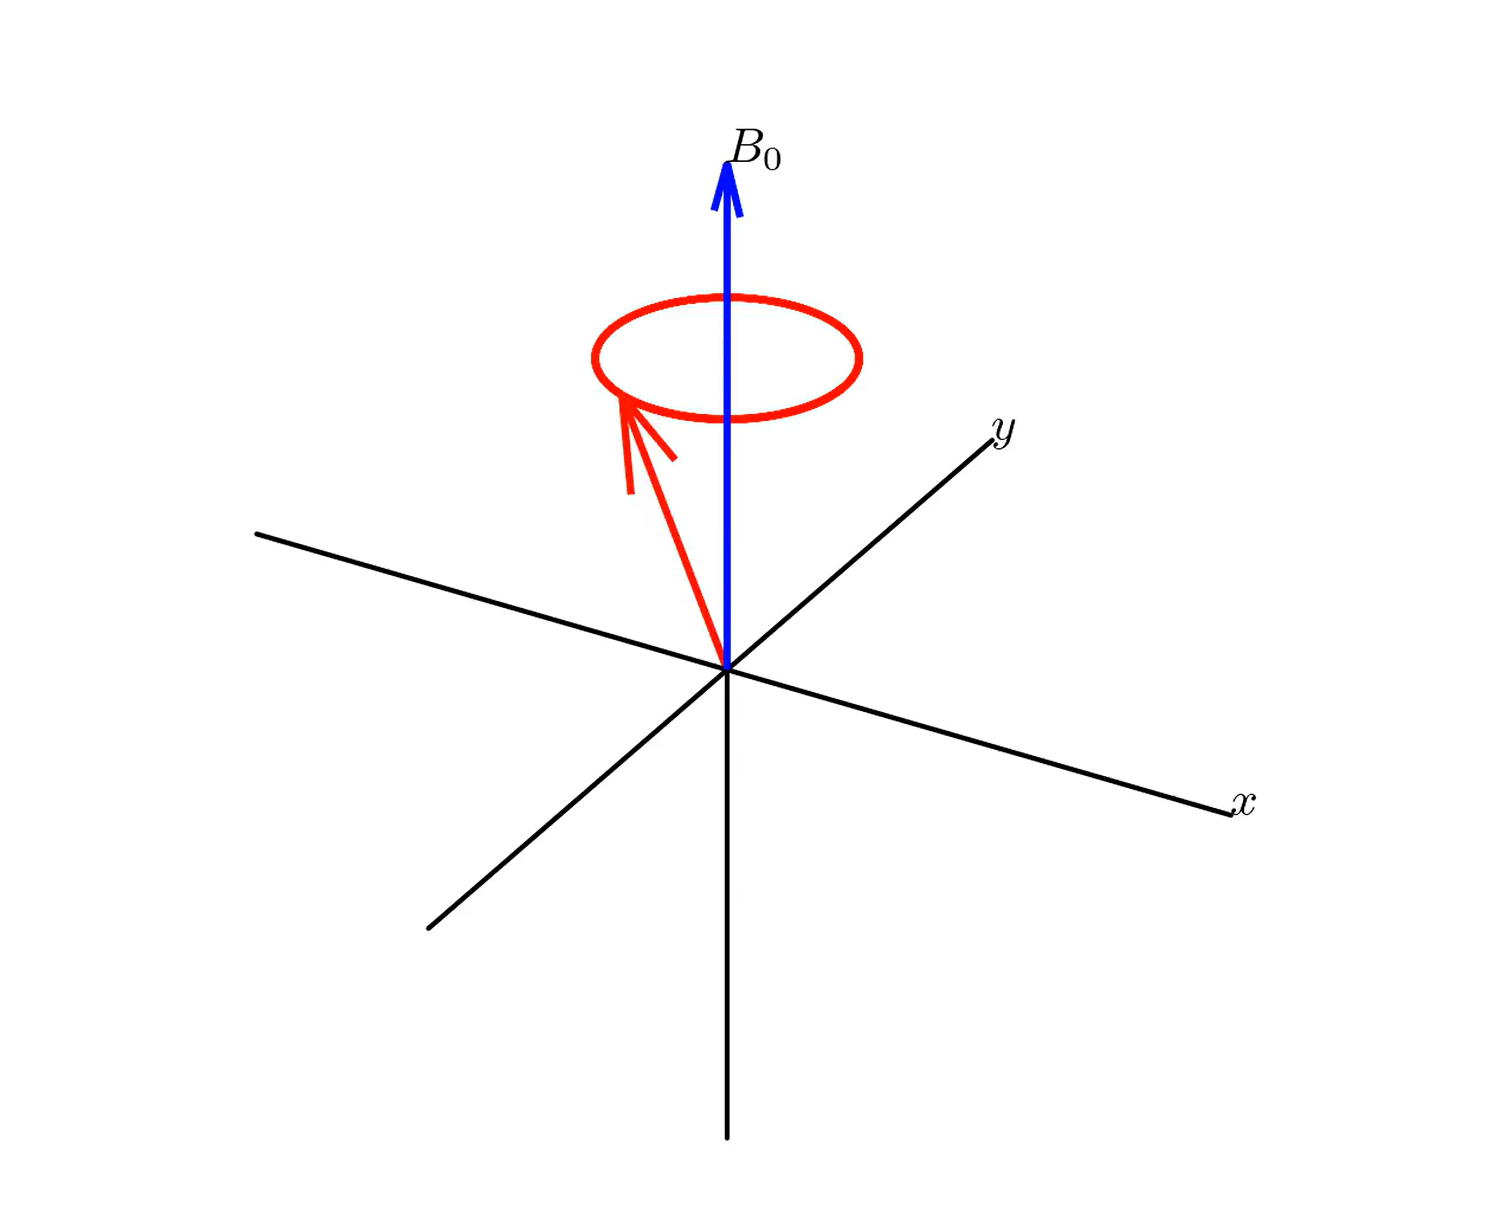
\includegraphics[width = 0.6\linewidth]{figs/larmor-precession.png}}
    \caption{Larmor precession about $\vec{B_0}$}
\end{figure}

$\theta$ characterizes the system, up to a phase,

\begin{gather*}
    \ket{\psi} = \cos\left(\sfrac{\theta}{2}\right)\ket{+}+ e^{i\phi}\sin\left(\sfrac{\theta}{2}\right) \ket{-}
\end{gather*}

These equations above can also be derived from a classical viewpoint; we can calculate the torque $\vec{\tau}  =\vec{ \mu }\times \vec{B_0}$ on the nucleus by the magnetic moment and use Newton's second law to derive a similar precession.










% ---------------------------------------------------------------------------- %

\subsection{\label{subsec:pulses} Net Magnetization and Relaxation}

The lower energy $E_+$ is the favored energy state; slightly more spins will align parallel to $\vec{B_0}$ as opposed to antiparallel. Using statistical mechanics, we can derive the expected number of $\ket{+}$ vs $\ket{-}$. Since this is a canonical two-state system, the ratio $\frac{N_+}{N_-}$ is equal to the ratio of the Boltzmann factors, yielding

\begin{equation}
    \frac{N_+}{N_-} = \exp\left(\frac{\gamma \hbar B_0}{k T}\right)
\end{equation}

This small difference produces a net longitudinal magnetization (in this context, ``longitudinal'' refers ``along the $B_0$ field''), which is the sum of the individual quantized spins of the sytem. \cite{lab-manual}

\begin{equation}
    M_z = \sum_i \gamma \hbar m_i = \frac{\hbar}{2} \gamma (N_+ - N_-)
\end{equation}

In equillibrium with our original magnetic field $B_0$, we expect a slight magnetization in the $+\hat{z}$ direction. However, if we were to apply another magnetic field briefly to this system, we would see a change in the net magnetization $\vec{M}(t)$. Eventually, the system will return back to its equillibrium state. In order to reach equillibrium, the system must give back energy to the surrounding lattice.

We are interested in understanding how long it takes for our system to reach equillibrium. In general, after a disturbance, the magnetization follows the Bloch equation, reproduced in Equation \ref{eqn:bloch-t1}.

\begin{equation}\label{eqn:bloch-t1}
    \frac{d \vec{M}(t)}{dt} = \frac{\vec{M}(t)-\vec{M_0}}{T_1}
\end{equation}

where $\vec{M_0}$ denotes the equillibrium magnetization. We refer to $T_1$ as the \textbf{spin-lattice relaxation time}. \cite{principles-resonance}

One can solve Equation \ref{eqn:bloch-t1} to yield

\begin{equation}\label{eqn:decay-eqn}
    M_{j}(t) = M_0 - (M_0 - M_i)e^{-\sfrac{t}{T_1}}
\end{equation}

where $M_0$ is the magnetization at equillibrium and $M_i$ is the initial magnetiztion.\cite{principles-resonance} This formulation will be useful later when performing experiments.










% ---------------------------------------------------------------------------- %

\subsection{\label{sec:tipping}Producing Transverse Magnetizations}



\subsubsection{Apply a Circularly Polarized Field}

So far, we have discussed the uniform $\vec{B_0}$ field. However, to produce a transverse magnetization (i.e. a magnetization in the x-y plane) we need to get creative. We will use a circularly polarized field,

\begin{equation}
    \vec{B_1}(t) = B_1\left[\cos(\omega_0t)\hat{x}+\sin(\omega_0t)\hat{y}\right]
\end{equation}

Note that $\vec{B_1}(t)$ oscillates at the Larmor frequency. Thus, the new Hamiltonian has an extra time-dependant term, still in the form of Equation \ref{eqn:base-hamiltonian}. Solving this Hamiltonian is beyond the scope of this lab report; however, we can still apply the classical torque result to obtain \cite{principles-resonance}

\begin{equation}
    \vec{\tau} = \vec{\mu} \times  \left[\vec{B_0}+\vec{B_1}(t)\right]
\end{equation}

by transforming into a rotating reference frame (rotating at the Larmor frequency), we find that the effective field becomes

\begin{equation}
    \vec{B}^* = (B_0 - \sfrac{\mu}{\gamma}) \hat{z}^*+ B_1 \hat{x}^*
\end{equation}

In this rotating frame, applying a circularly polarized magnetic field has the effect of ``tipping'' the magnetization into a transverse plane. Transforming back into the lab frame, we will observe the magnetization in the x-y plane still precessing about the z-axis.



\subsubsection{$\halfpi$ and $\pi$ pulses}

By applying $\vec{B_1}(t)$, we will create two types of pulses. We will first define a \textbf{$\halfpi$ pulse}, a pulse of $B_1(t)$ that will be applied for exactly long enough such that the magnetization is entirely in the $x-y$ plane. We will also define a \textbf{$\pi$ pulse}, a pulse that flips the magnetization from $+\hat{z}$ to $-\hat{z}$.


During a $\halfpi$ or $\pi$ pulse, we can plot the expectation $\langle \vec{S} \rangle  = (\langle S_x \rangle, \langle S_y \rangle, \langle S_z \rangle)$ over time, as shown in Figure \ref{fig:pulse-spirals}.


\begin{figure*}[htbp]
    \centering
    \begin{subfigure}{0.3\linewidth}
        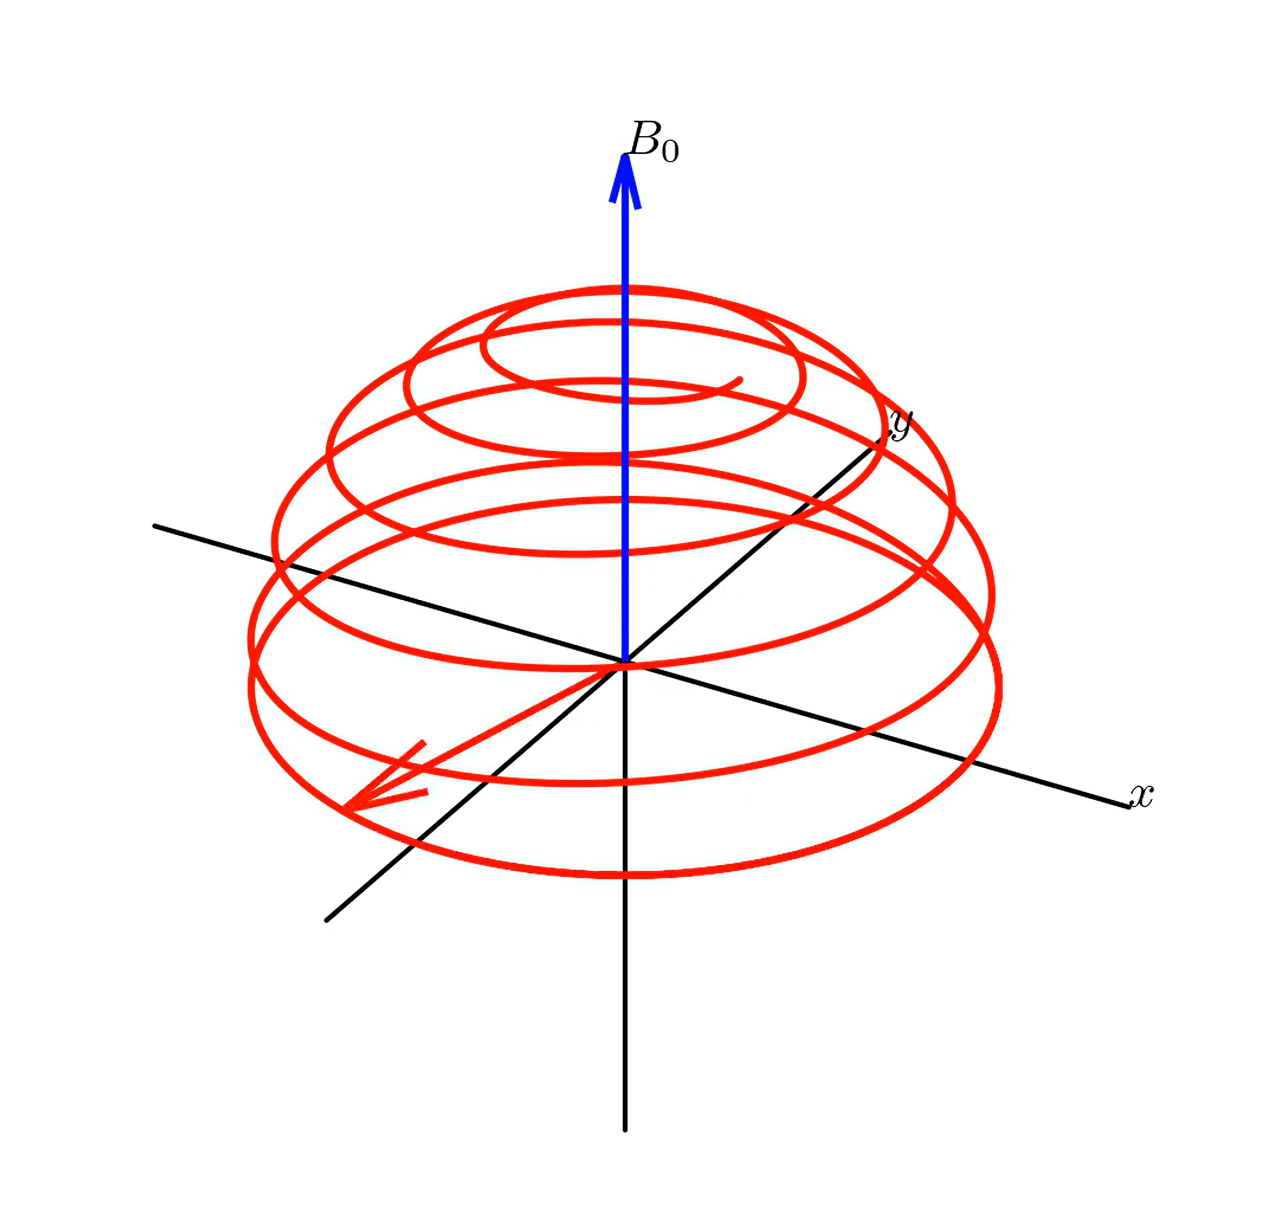
\includegraphics[width = \linewidth]{figs/pi-2-pulse.png}
        \caption{$\halfpi$ pulse produces transverse magentization}
    \end{subfigure}
    \begin{subfigure}{0.3\linewidth}
        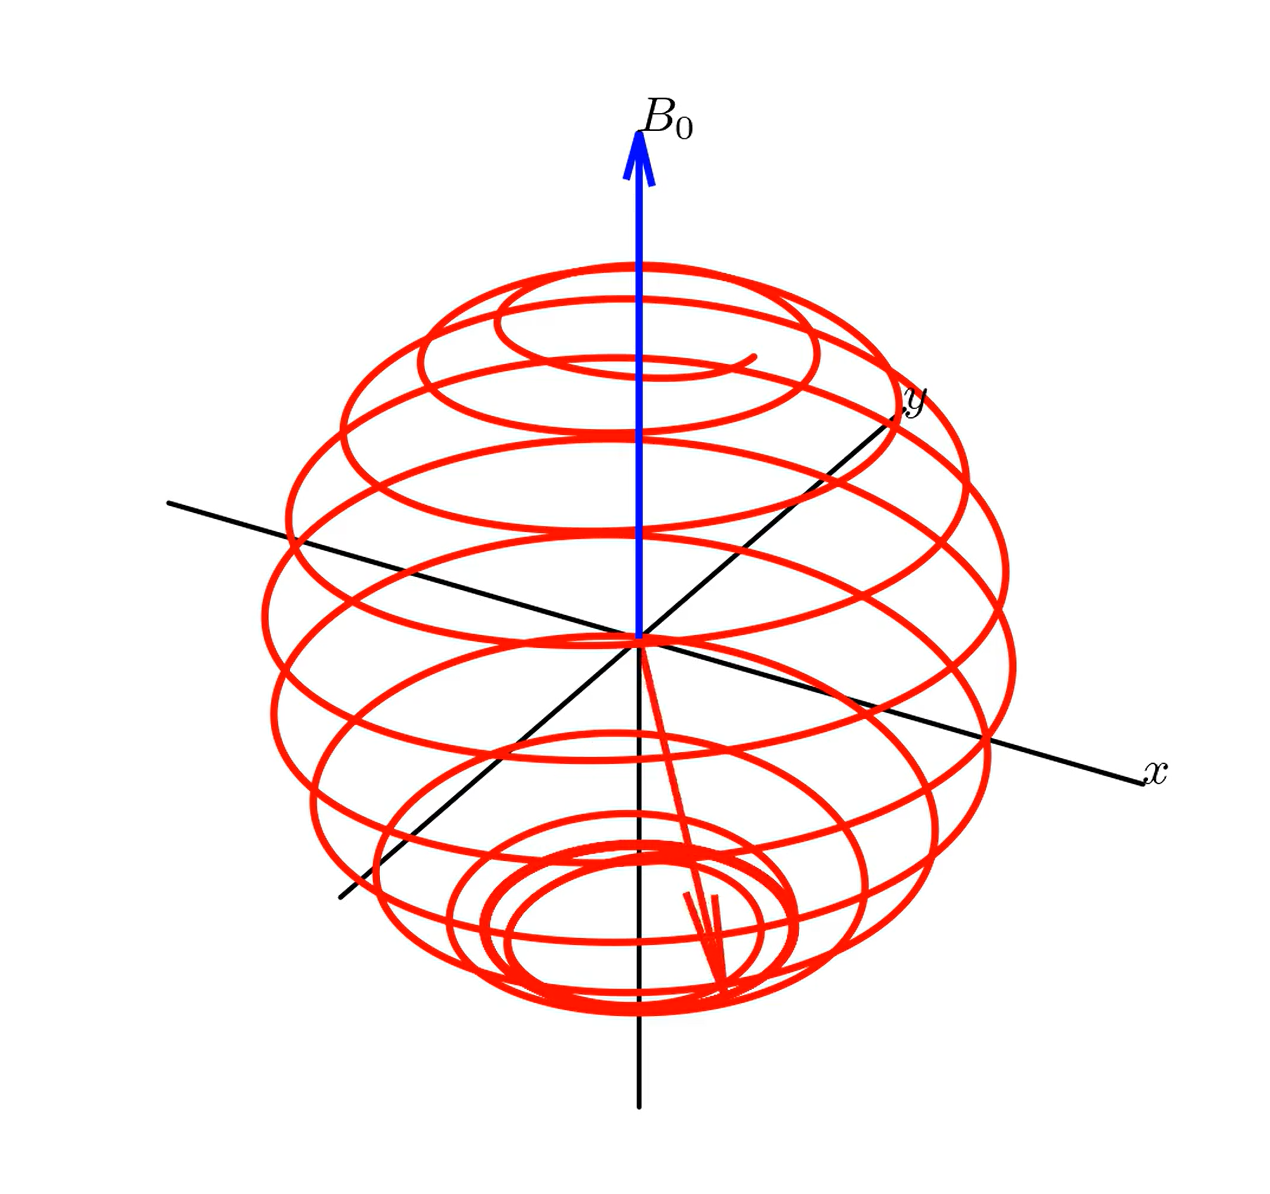
\includegraphics[width = \linewidth]{figs/pi-pulse.png}
        \caption{$\pi$ pulse flips magentization from $+\hat{z}$ to $-\hat{z}$}
    \end{subfigure}
    \caption{$\langle \vec{S} \rangle$ over time during a $\halfpi$ and $\pi$ pulse}\label{fig:pulse-spirals}
\end{figure*}

As a practical matter, the Larmor frequency generally lies in the radio frequency range for most atoms. As a result, the $\vec{B_1}(t)$ pulses are referred to as \textbf{RF pulses}.






% ---------------------------------------------------------------------------- %

\subsection{\label{sec:t2} Spin-Spin Relaxation}

Along with the decay of the transverse magnetization, we observe a different kind of decay; the decay of the relative phasing of all of the magnetic moments. After a $\halfpi$ pulse, the magnetic moments are in phase with each other---however, due to mutual interactions, these moments slowly turn out of phase. This dephasing is known as \textbf{spin-spin relaxation}, and obeys a similar relationship to Equation \ref{eqn:bloch-t1}. In particular, the external magnetic field denoted by $\vec{M}_0$ in Equation \ref{eqn:bloch-t1} is $\vec{0}$. Adapting this, we obtain Equation \ref{eqn:bloch-t2}.

\begin{equation}\label{eqn:bloch-t2}
    \frac{d\vec{M}_{x,y}}{dt} = \frac{\vec{M}_{x,y}}{T_2}
\end{equation}

Note that both Equation \ref{eqn:bloch-t1} and \ref{eqn:bloch-t2} are in the same form, following a familiar exponential curve.




% ---------------------------------------------------------------------------- %

\subsection{Free Induction Decay and $T_2^*$}

Suppose we apply a $\halfpi$ pulse to a system of nuclei; the net magnetization will be in the x-y plane. Further suppose we place this sample within a coil aligned in either the x or y direction. Since this magnetization is precessing at the Larmor frequency about \(\vec{B_0}\), the moment induces a change in flux in the coil, producing a periodic voltage we can measure.

This oscillation will decay according to Equations \ref{eqn:bloch-t1} and \ref{eqn:bloch-t2} as the magnetization becomes increasingly decoherent. The envelope of this decay is known as \textbf{free induction decay (FID)}.

The characteristic decay time constant of an FID signal depends not only on $T_1$ and $T_2$, but also local inhomogeneities in $\vec{B_0}$. We label the time constant obtained from all three factors $T_2^*$, which, with some simple algebra, we obtain as \cite{lab-manual}

\begin{equation}
    \frac{1}{T_2^*} = \frac{1}{T_1}+\frac{1}{T_2}+ \gamma \Delta B_0
\end{equation}

In order to directly measure $T_1$ and $T_2$, we must therefore get creative on our measurement techniques. By using specific pulse sequences (see Section IIA,B), the effects of the $\vec{\gamma \Delta B_0}$ can be mitigated and $T_1$ and $T_2$ can be isolated and calculated using Equations \ref{eqn:bloch-t1} and \ref{eqn:bloch-t2}, respectively.

















% ---------------------------------------------------------------------------- %
%                                    METHODS                                   %
% ---------------------------------------------------------------------------- %

\section{Apparatus and Experimental Procedure}

\begin{figure}
    \centering
    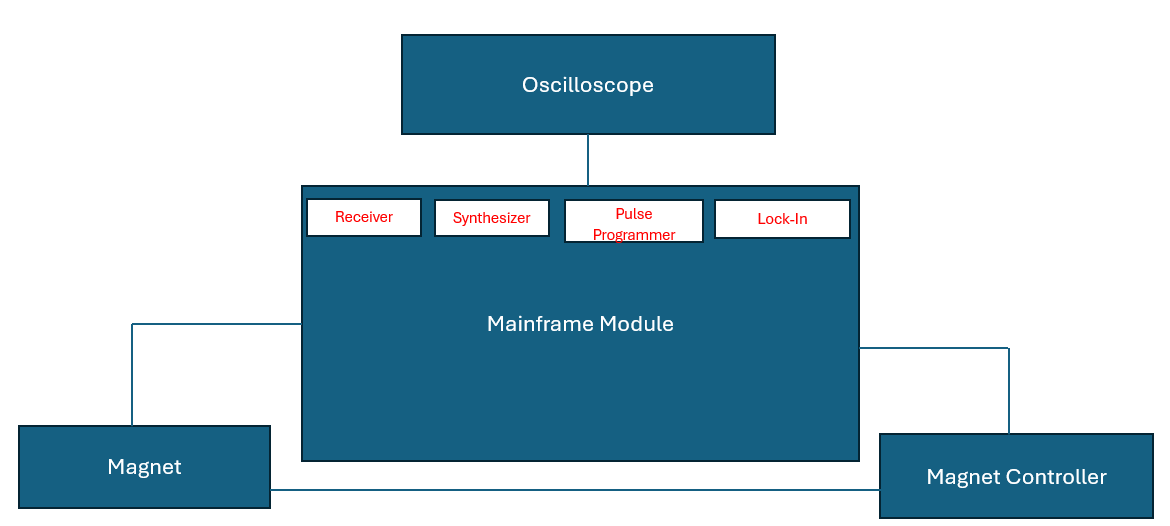
\includegraphics[width=\linewidth]{figs/Screenshot 2025-05-05 201540.png}
    \caption{TeachSpin NMR Apparatus}
    \label{apparatus}
\end{figure}

The apparatus for NMR experiments (Figure \ref{apparatus}) consists of a TeachSpin PS2-B Pulsed/CW NMR set and a Tektronix oscilloscope. The TeachSpin set comes with a \SI{0.49}{\tesla} permanent magnet, PS2 magnet temperature controller, and mainframe module with pulse programmer, synthesizer, receiver and lock-in amplifier. The synthesizer generates the signal that will be used to excite proton spins. The receiver reads the signal (specifically the envelope of the signal) from a pickup coil aligned with the x-axis of the permanent magnet; this coil outputs a voltage when proton spins produce a net change of flux. The oscilloscope then displays the output from the receiver. The pulse programmer allows for the length, period and delay time to be set for a pulse sequence. This will be critical in creating the sequences of $\halfpi$ and $\pi$ pulses needed to effectively measure NMR decay.

It is critical that the frequency of the RF signal be tuned to match the Larmor frequency of protons in the static magnetic field. For hydrogen, the Larmor frequecy is ~\SI{21}{\mega\hertz}.





% ---------------------------------------------------------------------------- %

\subsection{Measuring $T_1$ \label{sec:measure-t1}}

There are two traditional pulse sequences that allow for a T1 measurement: $\halfpi$ and $\pi-\halfpi$. By applying a single $\halfpi$ pulse, the net magnetization vector is tipped into the x-y plane, producing an FID signal. This signal quickly decays primarily due to the dephasing of individual spins, but also realignment of spins with the z-axis. Even after this signal disappears, the net magnetization vector is still decaying towards the z-axis. At any moment in time, another $\halfpi$ pulse can be applied. When this happens, any spins aligned with the z-axis are thrown back in the x-y plane and can be measured, while those in the x-y plane are rotated out of the measurement region. This means that by applying two $\halfpi$ pulses, one can effectively check the decay of net magnetization and characterize it with a time constant.

Alternatively, one can apply a $\pi$ pulse, which inverts the net magnetization to $-\hat{z}$. This produces a negligible FID signal, since the spins dephase before entering the measurement region (x-y plane). In spite of this, the net magnetization vector is still decaying towards $+\hat{z}$. At any moment in time, a $\halfpi$ pulse can be applied to, much like before, check the decay of the net magnetization. When the FID signal following a $\halfpi$ pulse is zero, half of the spins have decayed back to $+\hat{z}$. This is known as the \textbf{zero crossing time} and can be used to calculate the time constant of the decay. This method is preferred, since a null signal can easily be identified.





% ---------------------------------------------------------------------------- %

\subsection{Measuring $T_2$\label{sec:measure-t2}}

T2 measurements require a $\halfpi-\pi$ pulse sequence. The $\halfpi$ pulse tips the magnetization into the x-y plane, where the spins dephase due to inhomogeneities in the static magnetic field and spin-spin interactions. The goal in a T2 measurement is to isolate the spin-spin dephasing.  To do this, one must note that magnitude of spin dephasing is related to the strength of the static field it experiences. When a spin is kicked into the x-y plane, torque from the static magnetic field forces it to rotate in that plane. Spins in a stronger magnetic field rotate more quickly than ones in a weaker magnetic field, leading to aggressive dephasing. To mitigate this, a $\pi$ pulse is applied. The $\pi$ pulse essentially flips the direction of spin rotation, meaning all spins rotate back at roughly the same speed.

This leads to the `rephasing' of spins shortly after the pulse since spins that rotated more quickly following the $\halfpi$ pulse have a longer distance to travel on the way back after the $\pi$ pulse. This rephasing is known as a \textbf{spin echo}. If the inhomogeneous field were the only cause of dephasing, the magnitude of the rephased signal would equal the initial in phase signal. However, since spin-spin interactions are also dephasing spins, the rephased signal is slightly weaker. By applying multiple $\pi$ pulses after an initial $\halfpi$ pulse, one can track the decay in magnitude of the rephasing signal due to spin spin interactions and characterize it with a time constant, this time constant is T2.

It's important that the $\pi$ pulses are close together, since particle diffusion in a sample can cause a proton to move into a different magnetic field region. This would make the `rephasing' speed of the spin different from its initial `dephasing' speed, causing it to not rephase with other spins for reasons not related to the spin-spin interactions we seek to measure.










% ---------------------------------------------------------------------------- %
%                                    RESULTS                                   %
% ---------------------------------------------------------------------------- %

\section{Data and Analysis}




% ---------------------------------------------------------------------------- %

\subsection{Measuring $T_1$}

We start by a brief measurement of $T_1$ of mineral oil. We use the second ``preferred'' technique outlined in Section \ref{sec:measure-t1}. We apply a $\pi$ pulse and check the ratio of $\frac{N_+}{N_-}$ by applying a $\halfpi$. When we observe a null signal, we record the time between the $\pi$ and $\halfpi$ pulse.

No oscilloscope plot is available for this portion, because at null all you see is a straight line.

After a $\pi$ pulse, $M_z \rightarrow -M_z$, so at the zero-crossing, $\frac{N_+}{N_-} = 1$ and $M_z = 0$. One can then solve Equation \ref{eqn:decay-eqn} for $M_i = -M_z$ and $M_z(t_\text{crossing}) = 0$ to yield

\begin{equation}
    T_1 = \frac{t_\text{crossing}}{\ln(2)}
\end{equation}

For mineral oil, the obtained crossing point was

\begin{equation}
    t_\text{crossing} = \SI[separate-uncertainty = true]{34(.5)}{\milli\second}
\end{equation}

yielding

\begin{equation}
    T_1 = \SI[separate-uncertainty=true]{49.1(0.7)}{\milli\second}
\end{equation}








% ---------------------------------------------------------------------------- %

\subsection{Measuring $T_2$}

Now, we can attempt to measure $T_2$. We will use the $\halfpi-\pi$ sequence outlined in Section \ref{sec:measure-t2}. As mentioned previously, we apply one $\halfpi$ pulse, and then apply many $\pi$ pulses to isolate the spin-spin interaction (as opposed to effects caused by the inhomogeneity of the field). This produces spin echoes with decaying magnitude; this is known as the \textbf{Carr-Purcell sequence}.




\subsubsection{Simulating the Carr-Purcell Sequence}

As the individual spins precess around \(\vec{B_0}\), they will continue to rephase until reaching a maximum spin echo. This produces a periodic flux in the pickup coil with peaks, modeled by Equation \ref{eqn:simulation}

\begin{equation}\label{eqn:simulation}
    A(n) = A_0 \exp{\left( \sfrac{-t_n}{T_2} \right)} \cdot \left[ \tfrac{1}{2} \left(1 + \cos \left( \frac{2\pi n}{\mathrm{beatperiod}} \right)\right) \right]
\end{equation}

for $t_n = n \times \text{echo\_spacing}$. We define a continuous version by replacing the discrete index $n$ with $t/\text{echo\_spacing}$.

From a heuristic standpoint, this makes sense; we have a decaying envelope characterized by $\exp(\sfrac{t_n}{T_2})$ and beating following the periodic oscillation of the magnetization.

Plotting these results, we obtain Figure \ref{fig:simulation}.

\begin{figure}[htbp]
    \centering
    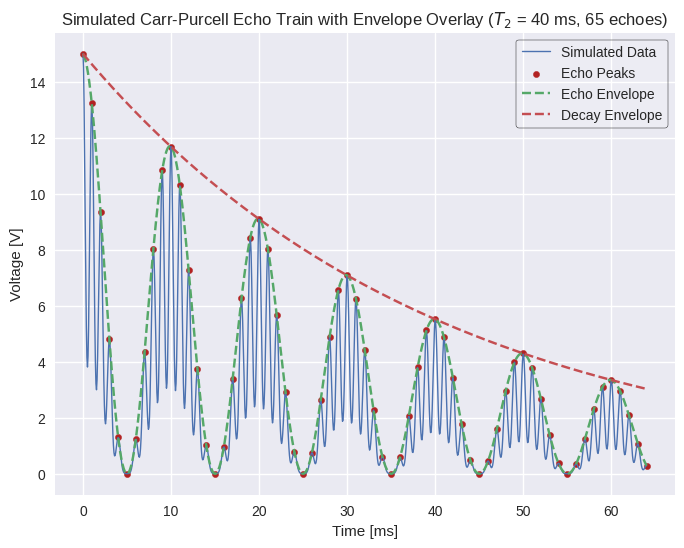
\includegraphics[width = 0.8\linewidth]{figs/purcell/simulation.png}
    \caption{Simulation of the beating behavior in a Carr-Purcell sequence with 60 $\pi$ pulses. Each echo is modeled as a Gaussian pulse. The echo amplitude decays exponentially (simulating $T_2$ decay) and is modulated by a cosine factor (to incorporate beating effects). Additionally, we overlay a smooth envelope curve that passes through the echo peak amplitudes.}\label{fig:simulation}
\end{figure}

Physically, in an idealized model we would ``see'' every individual rephasing event of the spins as a distinct, narrow pulse. However, in a real NMR detection system the output isn't the raw high-frequency signal — instead, the receiver circuitry (which includes mixers, rectifiers, and low-pass filters) performs envelope detection. This means that it extracts and outputs the overall amplitude envelope of the rapidly oscillating RF signal rather than the instantaneous voltage values.

The envelope represents the net decay or modulation of the transverse magnetization (affected by factors like $T_2$ and any beat modulation) rather than the fine time structure of each echo. As a result, the oscilloscope displays a smooth decaying curve rather than the ``spiky'' substructure seen in the simulation.






\subsubsection{Obtaining experimental values of $T_2$}

We will now create the Carr-Purcell with mineral oil. Apply a $\halfpi$ pulse and subsequent $\pi$ pulses to produce spin-echoes. Let \texttt{N} denote the number of $\pi$ pulses after a $\halfpi$ pulse. We perform this experiment with \texttt{N}=\{10, 20, 21, 50\}. We use varying separation times $\taucode$ between the pulses to get a feel for the procedure; the exact time isn't relavant for this part of the experiment, although minimizing times will produce more accurate results.


The envelope obeys Equation \ref{eqn:bloch-t2}; therefore, we fit an exponential to each of the experimental sets. We then obtain fitted time constants. These results are summarized in AHHHHHHHHHHHHHHHHHHHHHHHHHH EXPLAIN THIS MORE


% \begin{table}[htbp]
%     \centering
%     \caption{Relaxation parameters for mineral oil, corresponding to Figure \ref{fig:purcell/mineral_oil}.}
%     \label{tab:mineral_oil}
%     \begin{ruledtabular}
%         \begin{tabular}{ccc}
%             $N$ & $\tau$ (\si{\milli\second}) & $T_2$ (\si{\milli\second}) \\
%             \hline
%             10  & 0.0719 & 48.8 \\
%             20  & 0.0342 & 41.1 \\
%             21  & 0.164  & 44.7 \\
%             50  & 0.0882 & 41.3 \\
%         \end{tabular}
%     \end{ruledtabular}
% \end{table}

% \begin{table}[htbp]
%     \centering
%     \caption{Relaxation parameters for glycerin, corresponding to Figure \ref{fig:purcell/glycerin}.}
%     \label{tab:glycerin}
%     \begin{ruledtabular}
%         \begin{tabular}{ccc}
%             $N$ & $\tau$ (\si{\milli\second}) & $T_2$ (\si{\milli\second}) \\
%             \hline
%             20  & 0.0761 & 27.3 \\
%             31  & 0.0780 & 27.7 \\
%             35  & 0.0204 & 28.5 \\
%             50  & 0.0196 & 27.6 \\
%         \end{tabular}
%     \end{ruledtabular}
% \end{table}

% \begin{table}[htbp]
%     \centering
%     \caption{Relaxation parameters for deionized water, corresponding to Figure \ref{fig:purcell/water}.}
%     \label{tab:water}
%     \begin{ruledtabular}
%         \begin{tabular}{ccc}
%             $N$  & $\tau$ (\si{\milli\second}) & $T_2$ (\si{\milli\second}) \\
%             \hline
%             98   & 1.16   & 777 \\
%             100  & 0.594  & 926 \\
%         \end{tabular}
%     \end{ruledtabular}
% \end{table}

% \begin{table}[htbp]
%     \centering
%     \caption{Relaxation parameters for three compounds.}
%     \label{tab:relaxation-all}
%     \sisetup{table-format=2.3}  % align decimals
%     \begin{tabular}{l S[table-format=2.0] S[table-format=1.4] S[table-format=3.1]}
%         \toprule
%         Compound & {$N$} & {$\tau$ (\si{\milli\second})} & {$T_2$ (\si{\milli\second})} \\
%         \midrule
%         \multirow{4}{*}{Mineral oil}
%         & 10  & 0.0719 &  48.8 \\
%         & 20  & 0.0342 &  41.1 \\
%         & 21  & 0.1640 &  44.7 \\
%         & 50  & 0.0882 &  41.3 \\[1ex]
%         \multirow{4}{*}{Glycerin}
%         & 20  & 0.0761 &  27.3 \\
%         & 31  & 0.0780 &  27.7 \\
%         & 35  & 0.0204 &  28.5 \\
%         & 50  & 0.0196 &  27.6 \\[1ex]
%         \multirow{2}{*}{DI water}
%         & 98  & 1.1600 & 777.0 \\
%         & 100 & 0.5940 & 926.0 \\
%         \bottomrule
%     \end{tabular}
% \end{table}


\


\

% \begin{tabular*}{0.9\linewidth}{@{\extracolsep{\fill}}l c c c@{}}
%     \toprule
%     Compound       & $N$  & $\tau$ (\si{\milli\second}) & $T_2$ (\si{\milli\second}) \\
%     \midrule
%     Mineral oil    & 10   & 0.0719                      & 48.8                       \\
%     & 20   & 0.0342                      & 41.1                       \\
%     & 21   & 0.1640                      & 44.7                       \\
%     & 50   & 0.0882                      & 41.3                       \\
%     \addlinespace
%     \hline
%     \addlinespace
%     Glycerin       & 20   & 0.0761                      & 27.3                       \\
%     & 31   & 0.0780                      & 27.7                       \\
%     & 35   & 0.0204                      & 28.5                       \\
%     & 50   & 0.0196                      & 27.6                       \\
%     \addlinespace
%     \hline
%     \addlinespace
%     Deionized water& 98   & 1.1600                      & 777.0                      \\
%     & 100  & 0.5940                      & 926.0                      \\
%     \bottomrule
% \end{tabular*}



\begin{table}[htbp]
    \centering
    \caption{Relaxation parameters for mineral oil, glycerin, and deionized water.}
    \label{tab:relaxation-all}
    \begin{tabular*}{0.9\linewidth}{@{\extracolsep{\fill}}l c c c@{}}
        \toprule
        Compound        & $N$   & $\tau$ (\si{\milli\second}) & $T_2$ (\si{\milli\second}) \\
        \midrule
        Mineral oil     & 10    & 0.0719                      & 48.8                        \\
        & 20    & 0.0342                      & 41.1                        \\
        & 21    & 0.1640                      & 44.7                        \\
        & 50    & 0.0882                      & 41.3                        \\
        \addlinespace
        \midrule
        \addlinespace
        Glycerin        & 20    & 0.0761                      & 27.3                        \\
        & 31    & 0.0780                      & 27.7                        \\
        & 35    & 0.0204                      & 28.5                        \\
        & 50    & 0.0196                      & 27.6                        \\
        \addlinespace
        \midrule
        \addlinespace
        Deionized water & 98    & 1.1600                      & 777.0                       \\
        & 100   & 0.5940                      & 926.0                       \\
        \bottomrule
    \end{tabular*}
\end{table}



\begin{table}[htbp]
    \centering
    \caption{Mean and standard deviation of \(T_2\) for each compound.}
    \label{tab:t2-stats}
    \setlength{\tabcolsep}{12pt}   % default is 6pt; try 8pt, 10pt, 12pt...
    \begin{tabular}{l c c}
        \toprule
        Compound      & Mean (\si{\milli\second}) & Std.\ dev.\ (\si{\milli\second}) \\
        \midrule
        Glycerin      & 27.8    & 0.509  \\
        Mineral oil   & 44.0    & 3.61   \\
        Water         & 851     & 105    \\
        \bottomrule
    \end{tabular}
\end{table}




% ---------------------------------------------------------------------------- %
%                                  CONCLUSION                                  %
% ---------------------------------------------------------------------------- %


\section{Conclusion}

In this report, we discussed our efforts to
measure spin-lattice (T1) and spin-spin (T2) relaxation
times for mineral oil, glycerin, and distilled water. We also discussed the different RF
pulse sequences that allow for best T1 and T2 measurements. Using the zero-crossing method for measuring T1 we measured 49.1, 40.4, and 1880 ms as the T1 relaxation times for mineral oil, glycerin and water, respectively. By using the Carr-Purcell sequence method, we measured 44, 28, and 851 ms as the T2 relaxation times, respectively. The significant differences between T1 and T2 times for different substances emphasizes the usefulness of NMR for material characterization.


























% ---------------------------------------------------------------------------- %
%                                    FOOTER                                    %
% ---------------------------------------------------------------------------- %


\section{References}

% The \nocite command causes all entries in a bibliography to be printed out
% whether or not they are actually referenced in the text. This is appropriate
% for the sample file to show the different styles of references, but authors
% most likely will not want to use it.
\nocite{*}

\bibliography{appsamp.bib} % Produces the bibliography via BibTeX.










% ---------------------------------------------------------------------------- %
%                               APPENDIX: GRAPHS                               %
% ---------------------------------------------------------------------------- %


\clearpage

\onecolumngrid
\appendix
\section{Full-Size Purcell Plots for Mineral Oil, Glycerin, and DI Water}

\begin{figure*}[htbp]
    \centering
    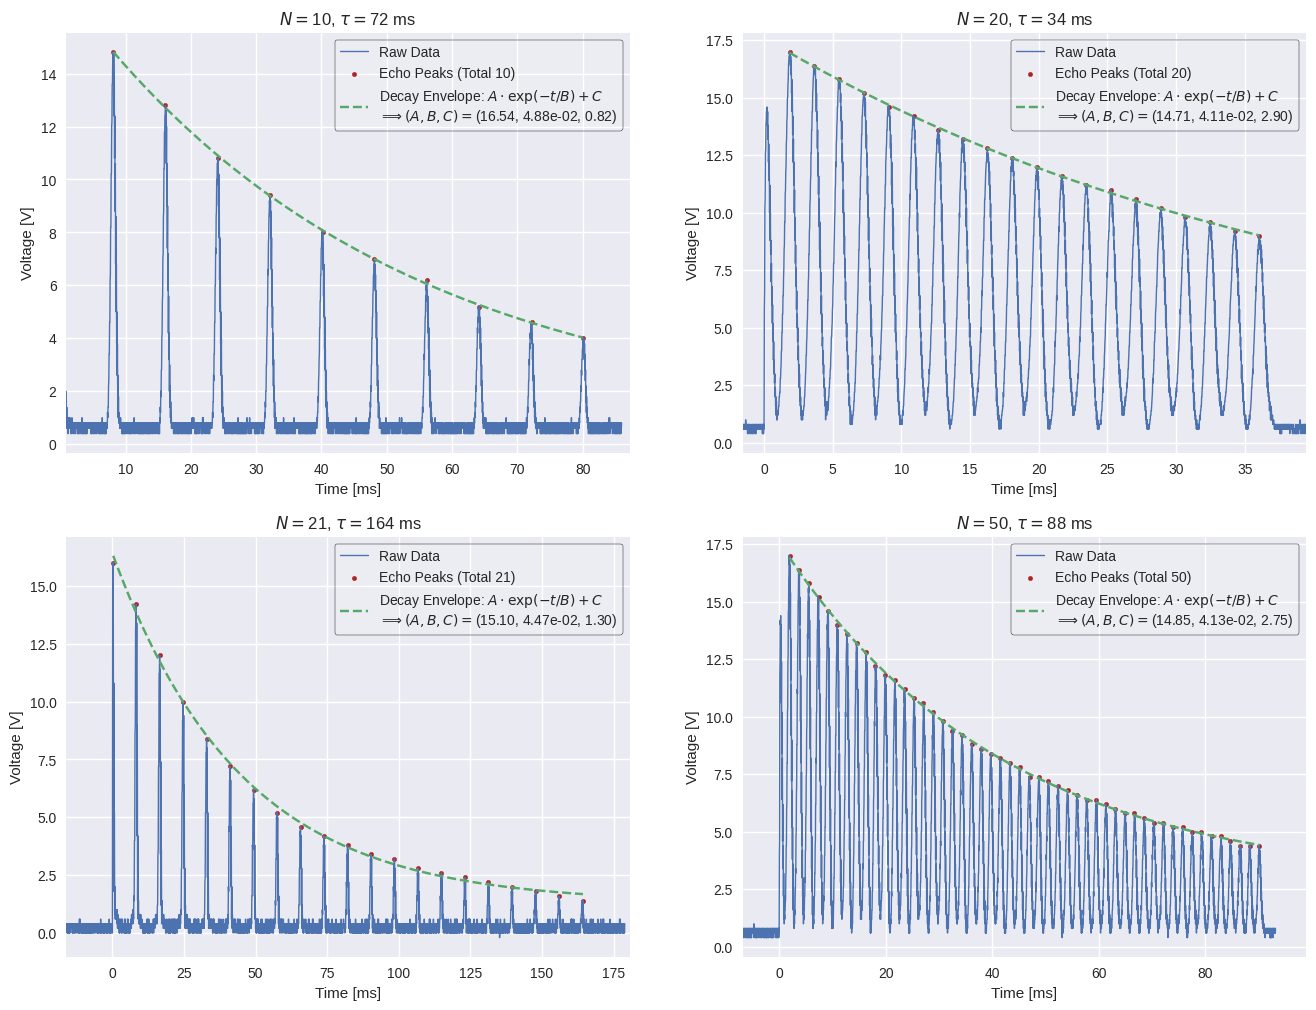
\includegraphics[width=\textwidth]{figs/purcell/mineral_oil.png}
    \caption{Carr-Purcell sequences with various $N, \tau$ for mineral oil.}
    \label{fig:purcell/mineral_oil}
\end{figure*}

\begin{figure*}[htbp]
    \centering
    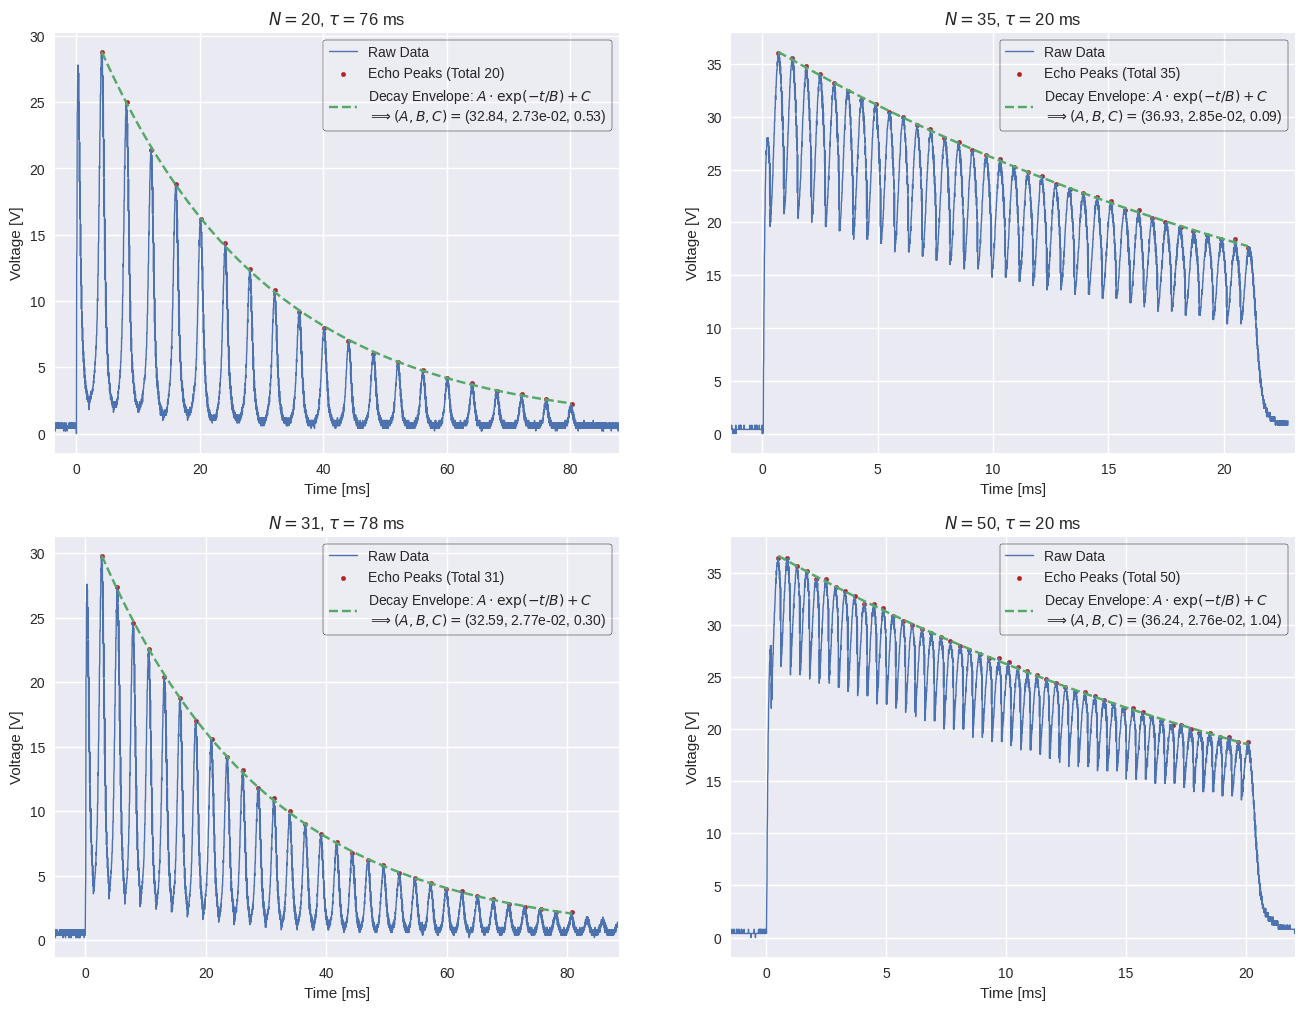
\includegraphics[width=\textwidth]{figs/purcell/glycerin.png}
    \caption{Carr-Purcell sequences with various $N, \tau$ for glycerin.}
    \label{fig:purcell/glycerin}
\end{figure*}

\begin{figure*}[htbp]
    \centering
    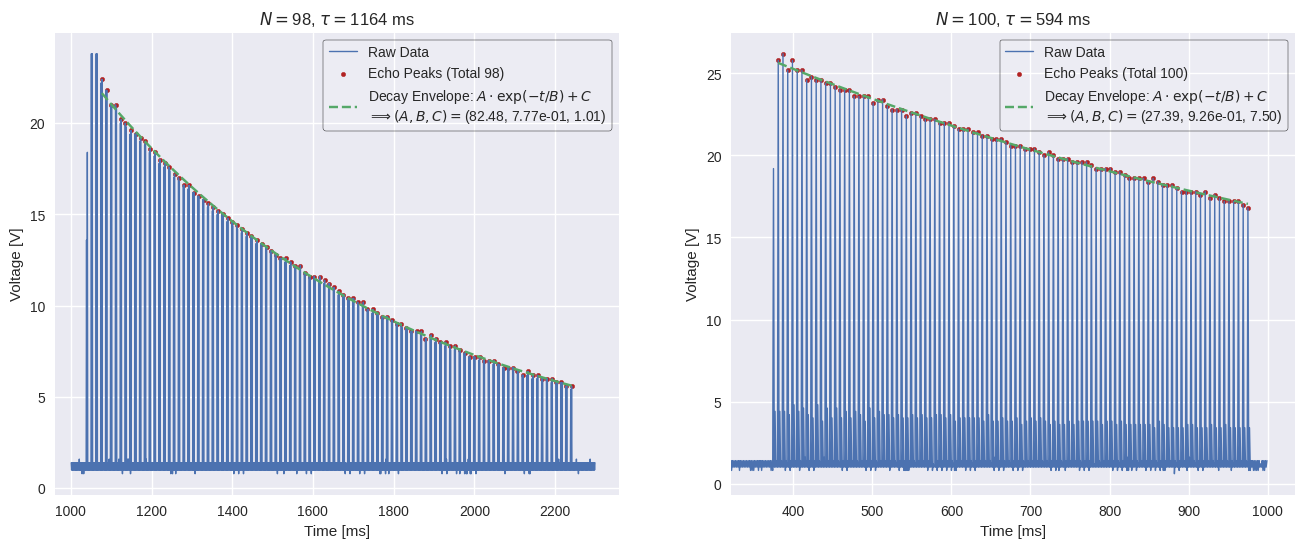
\includegraphics[width=\textwidth]{figs/purcell/water.png}
    \caption{Carr-Purcell sequences with various $N, \tau$ for deionized water.}
    \label{fig:purcell/water}
\end{figure*}


\twocolumngrid



















% ---------------------------------------------------------------------------- %

\end{document}
